% Topologies of the shipped examples, drawn with the same conventions as the
% Feynman-rules figure: the SK branch of a vertex is carried by its fill colour, black = + and
% white = -, gray = general. Vertices carry the conformal time and the vertex energy, propagators
% are drawn as plain unarrowed strokes carrying momentum labels, external legs end in small squares.
\documentclass[tikz,border=8pt]{standalone}
\usetikzlibrary{calc,arrows.meta}
\begin{document}
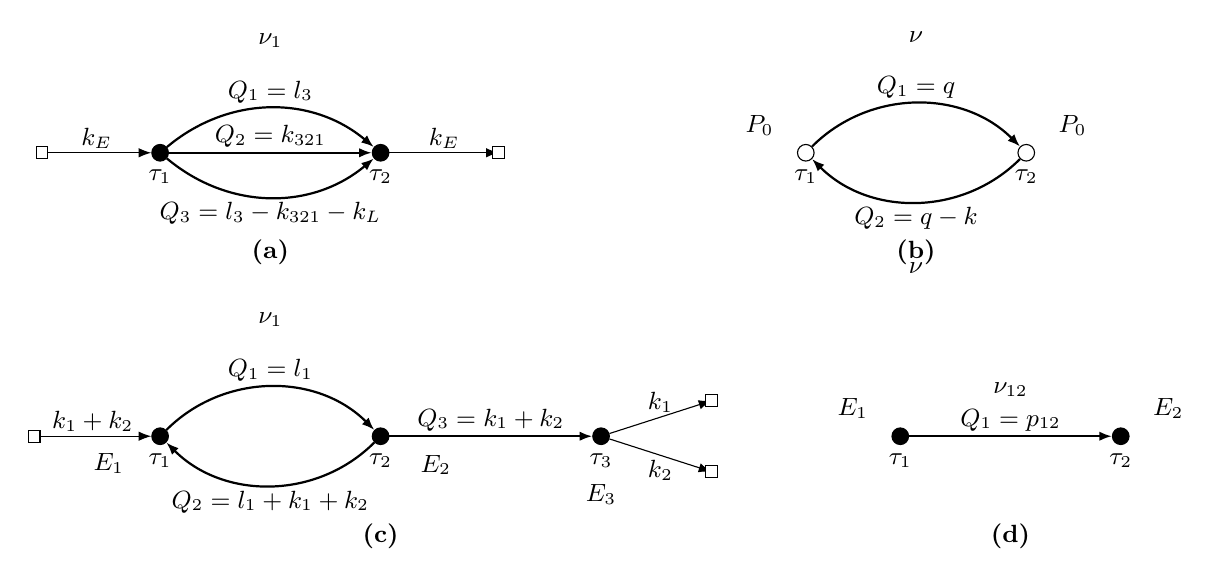
\begin{tikzpicture}[
  every node/.style={inner sep=1.5pt,font=\small},
  vertexP/.style={circle,fill=black,draw=black,minimum size=6pt,inner sep=0pt},
  vertexM/.style={circle,fill=white,draw=black,minimum size=6pt,inner sep=0pt},
  arr/.style={-{Latex[length=1.6mm]},thick},
  ext/.style={-{Latex[length=1.6mm]}},
  pnl/.style={font=\small\bfseries},
  yscale=1.0
]
% ================= (a) single massive sunrise =================
\begin{scope}[shift={(0,0)}]
  \node[vertexP] (v1) at (0,0) {};
  \node[vertexP] (v2) at (2.8,0) {};
  \draw[arr] (v1) to[bend left=40] node[above] {$Q_1=l_3$} (v2);
  \draw[arr] (v1) -- node[above] {$Q_2=k_{321}$} (v2);
  \draw[arr] (v1) to[bend right=40] node[below] {$Q_3=l_3-k_{321}-k_L$} (v2);
  \node[anchor=south] at (1.4,1.28) {$\nu_1$};
  \draw[ext] (-1.5,0) -- (v1) node[midway,above] {$k_E$};
  \filldraw[fill=white,draw=black] ($(0,0)+(-1.5,0)+(-0.075,0.075)$) rectangle ++(0.15,-0.15);
  \draw[ext] (v2) -- (4.3,0) node[midway,above] {$k_E$};
  \filldraw[fill=white,draw=black] ($(4.3,0)+(-0.075,0.075)$) rectangle ++(0.15,-0.15);
  \node[anchor=north] at (0,-0.16) {$\tau_1$};
  \node[anchor=north] at (2.8,-0.16) {$\tau_2$};
  \node[pnl,anchor=north] at (1.4,-1.05) {(a)};
\end{scope}
% ================= (b) pure massive bubble =================
\begin{scope}[shift={(8.2,0)}]
  \node[vertexM] (v1) at (0,0) {};
  \node[vertexM] (v2) at (2.8,0) {};
  \draw[arr] (v1) to[bend left=45] node[above] {$Q_1=q$} (v2);
  \draw[arr] (v2) to[bend left=45] node[below] {$Q_2=q-k$} (v1);
  \node[anchor=south] at (1.4,1.34) {$\nu$};
  \node[anchor=north] at (1.4,-1.34) {$\nu$};
  \node[anchor=north] at (0,-0.16) {$\tau_1$};
  \node[anchor=north] at (2.8,-0.16) {$\tau_2$};
  \node[anchor=east] at (-0.35,0.35) {$P_0$};
  \node[anchor=west] at (3.15,0.35) {$P_0$};
  \node[pnl,anchor=north] at (1.4,-1.05) {(b)};
\end{scope}
% ================= (c) mix bubble + tree =================
\begin{scope}[shift={(0,-3.6)}]
  \node[vertexP] (w1) at (0,0) {};
  \node[vertexP] (w2) at (2.8,0) {};
  \node[vertexP] (w3) at (5.6,0) {};
  \draw[arr] (w1) to[bend left=45] node[above] {$Q_1=l_1$} (w2);
  \draw[arr] (w2) to[bend left=45] node[below] {$Q_2=l_1+k_1+k_2$} (w1);
  \draw[arr] (w2) -- node[above] {$Q_3=k_1+k_2$} (w3);
  \node[anchor=south] at (1.4,1.34) {$\nu_1$};
  \draw[ext] (-1.6,0) -- (w1) node[midway,above] {$k_1+k_2$};
  \filldraw[fill=white,draw=black] ($(-1.6,0)+(-0.075,0.075)$) rectangle ++(0.15,-0.15);
  \draw[ext] (w3) -- (7.0,0.45) node[midway,above] {$k_1$};
  \filldraw[fill=white,draw=black] ($(7.0,0.45)+(-0.075,0.075)$) rectangle ++(0.15,-0.15);
  \draw[ext] (w3) -- (7.0,-0.45) node[midway,below] {$k_2$};
  \filldraw[fill=white,draw=black] ($(7.0,-0.45)+(-0.075,0.075)$) rectangle ++(0.15,-0.15);
  \node[anchor=north] at (0,-0.16) {$\tau_1$};
  \node[anchor=north] at (2.8,-0.16) {$\tau_2$};
  \node[anchor=north] at (5.6,-0.16) {$\tau_3$};
  \node[anchor=east] at (-0.4,-0.35) {$E_1$};
  \node[anchor=north] at (3.5,-0.18) {$E_2$};
  \node[anchor=north] at (5.6,-0.55) {$E_3$};
  \node[pnl,anchor=north] at (2.8,-1.05) {(c)};
\end{scope}
% ================= (d) two-vertex tree =================
\begin{scope}[shift={(9.4,-3.6)}]
  \node[vertexP] (u1) at (0,0) {};
  \node[vertexP] (u2) at (2.8,0) {};
  \draw[arr] (u1) -- node[above] {$Q_1=p_{12}$} (u2);
  \node[anchor=south] at (1.4,0.45) {$\nu_{12}$};
  \node[anchor=north] at (0,-0.16) {$\tau_1$};
  \node[anchor=north] at (2.8,-0.16) {$\tau_2$};
  \node[anchor=east] at (-0.35,0.35) {$E_1$};
  \node[anchor=west] at (3.15,0.35) {$E_2$};
  \node[pnl,anchor=north] at (1.4,-1.05) {(d)};
\end{scope}
\end{tikzpicture}
\end{document}
